\documentclass[lettersize,journal]{IEEEtran}
\usepackage{amsmath,amsfonts}
\usepackage{algorithmic}
\usepackage{array}
\usepackage[caption=false,font=normalsize,labelfont=sf,textfont=sf]{subfig}
\usepackage{textcomp}
\usepackage{stfloats}
\usepackage{url}
\usepackage{verbatim}
\usepackage{graphicx}
\hyphenation{op-tical net-works semi-conduc-tor IEEE-Xplore}
\def\BibTeX{{\rm B\kern-.05em{\sc i\kern-.025em b}\kern-.08em
    T\kern-.1667em\lower.7ex\hbox{E}\kern-.125emX}}
\usepackage{balance}
\begin{document}
\title{Blind Spectral Sensing based on Recurrence Plots on FFT for Cognitive Radio}
\author{Luciana De Micco and Maximiliano Antonelli 
\thanks{Manuscript created xx, 202x revised x; accepted xx Date of publication xx; date of current version}
\thanks{L. De Micco and M. Antonelli are with Institute of Scientific and Technological Research in Electronics (ICYTE) and  Engineering Faculty of the National University of Mar del Plata (UNMDP) and National Scientific and Technical Research Council (CONICET). Mar del Plata, Buenos Aires, Argentina, (email: \{ldemicco;maxanto\}@fi.mdp.edu.ar)}
\thanks{This research was funded by the National Scientific and Technical Research Council (PIP11220170100553CO), Agencia Nacional de Promoción Científica y Tecnológica (PICT2019-3024), Faculty of Engineering of the National University of Mar del Plata (FI-UNMDP).}}

\markboth{Journal of \LaTeX\ Class Files,~Vol.~, No.~,  ~20}%
{How to Use the IEEEtran \LaTeX \ Templates}

\maketitle

\begin{abstract}

Spectral sensing is a crucial step in the performance of Cognitive Radio (CR) systems. Among the existing methods, very few are capable of working in a ``blind'' way (neither information from the primary user (PU) is needed, nor the noise in the channel). This letter presents a blind spectral sensing method that is based on the Diagonal lines quantifier of the Recurrence Plots applied on the Fourier transform (FFT) of the received signal. Simulations were carried out showing that the proposed method presents better performance than the existing ones. 
\end{abstract}

\begin{IEEEkeywords}
Diagonal Line Lengths, Cognitive Radio, Recurrence Plots, Channel Sensing, Blind Spectral Sensing.
\end{IEEEkeywords}

\section{Introduction}
Many frequency bands have low usage by their licensed users. This waste of the spectrum together with the growing demand in wireless communications led to the emergence of the Cognitive Radio technique \cite{Arjoune2019}. The CR technique was presented by Mitola as a solution to the growing spectral demand due to the great increase in wireless communications \cite{Mitola2000}.
In a CR network, a secondary user can transmit over a channel that is assigned to a licensed user (from now on primary users or PU) when the primary user is not transmitting. Therefore, detecting the presence of primary users, especially at low signal-to-noise ratios (SNR), is critical in this type of network. Within the existing techniques, the adapted filter technique \cite{Bhargavi2010} and those based on cyclo-stationary detection \cite{Chen2007} show the best performances. However, they require information from the primary user and the level of noise present in the channel, besides they have a very high computational complexity \cite{Mehdawi2014}.
On the other hand, the techniques based on energy detection  \cite{Yadav2016} are the most used given their simplicity, in addition to not requiring information on the modulation of the primary user. However, they have the disadvantage of requiring \textit{a priori} knowledge of the noise power in the channel. With this uncertainty, their performance significantly worsens. There exist methods that need prior knowledge of neither the noise power in the channel nor the modulation of the primary user. These methods are known as blind methods. Such is the case of detection based on covariance \cite{Jin2012} and on eigenvalues \cite{Zeng2009}, the latter for cooperative receptors.

In this letter we propose a blind spectral sensing technique for CR, based on a quantifier from the Recurrence Plots, that is applied to the Fourier transform of the received signal. This work is a  continuation of \cite{Antonelli2021} in which a first approximation of the proposed method was made. Here, an improvement to the quantifier is achieved by incorporating the FFT into the method. Also, comparisons with existing techniques are incorporated to evidence that the proposed method outperforms them.
We get the Closed-form expression to the optimal threshold of local detection to get a trade-off between missed detection probability and false alarm probability.

\section{Spectral Sensing Considerations}
The first step for sensing the spectrum is to tune the channel of interest using a local oscillator and bring the incoming signal to an intermediate frequency. Then, the received signal is sampled at $f_s$ frequency, obtaining a sequence $y_k$ which will enter the quantifier.

When the channel is available ($H_0$), the sequence $y_k$ is a random variable with Gaussian Probability Density Function (PDF). Otherwise, when the channel is busy ($H_1$), the PU signal plus Gaussian noise will be sampled. In general, it is required to detect signals under very low SNR conditions, then the PDF under $H_1$ can also be approximate to  a Gaussian PDF. By applying the quantifiers to the incoming sequence, a random variable, $z_k$, is obtained, which will present a new PDF, as seen in Fig. \ref{fig:pdfs}. 

The next step for sensing is to establish a threshold value $z_{th}$, which will be compared with each $z_k$ to determine whether a PU signal is present or not. If $z_k>z_{th}$ it will be determined that there is a PU signal, otherwise the channel will be taken as available. This threshold is established considering what probability of detecting the PU signal erroneously is willing to accept ($P_{FA}$), taking into account that a lower $P_{FA}$  implies a lower probability of detecting the PU signal, $P_d$ (see Fig. \ref{fig:pdfs}). The area under the curve of the noise-only PDF ($H_0$) from $z_{th}$ to infinity will be $P_{FA}$. Therefore,  it is necessary to know this PDF to set the threshold. In the case of blind sensors, the PDF under $H_0$ does not change its characteristics with the noise power present in the channel. Then, it is possible to set a threshold independently of the noise power. In the case of energy detection based sensors, the mean value and variance of their PDFs do depend on the noise power, so a different threshold must be set for each SNR.

The distributions of the random variable $z_k$ (at the output of the quantifier) determine the performance that the sensor will have. This performance is generally quantified by the ROC curve (Receiver Operation Characteristics) \cite{Brown2005} that plots $P_{FA}$ vs $P_{d}$. The further apart these PDFs are (this is the more different mean values and the lower variance), the better the performance the system will present. In that situation, the ROC curve will deviate further from the $P_ {FA} = P_ {d}$ diagonal. Of course, the higher the SNR used, the more separate the PDFs will be.

\begin{figure}[htbp]
    \centerline{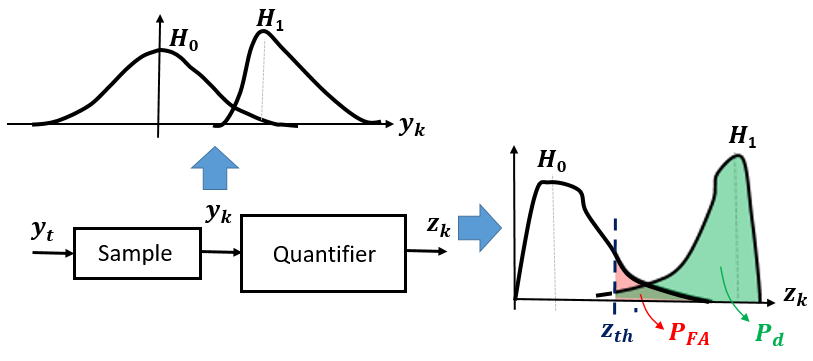
\includegraphics[width=\columnwidth]{pdfs.png}}
    \caption{Evolution diagram of the PDFs of the incoming signal to the quantifier.}
    \label{fig:pdfs}
\end{figure}

\section{$L_{FFT}$ quantifier}\label{secRecurrencePlots}
The proposed quantifier comes from the Recurrence Plots methods (RP) \cite{Eckmann1987}. These diagrams allow visualizing repetitions in the evolution of the state space of a sequence of data.
The repetition or recurrence of a state (considering an error $\epsilon$) is its appearance at two different times  $t_i,\,t_j$, and is represented by a point in the diagram.
The so-called recurrence function can be expressed mathematically:
\begin{equation}
    \mathbf{R}_{i,j}=\Theta\left(\varepsilon-\|\overrightarrow{x}_i-
    \overrightarrow{x}_j\|\right),\quad \label{eq:eq_rec}
\end{equation}
with $\overrightarrow{x}_i\in \mathbb{R}^{m}$ and $i,j=1,\cdots,N$. $N$ is the number of considered discrete states $\overrightarrow{x}_i$, $\|\bullet\|$ is a norm, and $\Theta(\bullet)$ is the Heaviside function.
%We here adopt the criteria used in \cite{Li2004}, where the expected error is calculated as $\epsilon = std(x_k)$.
Deterministic processes originate diagonal lines in the RP, whereas uncorrelated processes generate isolated points.
Several quantifiers that are based on the RP can be defined. They are used to obtain some description of the underlying system. 
In this case, the mean length of the diagonal lines was chosen since it proved to be the most sensitive to the presence of the PU signal:
\begin{equation}
    \label{eq:L}
    L=\frac{\sum_{l=l_{min}}^{N} l \cdot P(\varepsilon,l)}{\sum_{l=l_{min}}^{N}P(\varepsilon,l)}\;;
\end{equation}
where $l_{min}$ is the minimum length of the diagonal lines considered, $l$ is the length of each diagonal line on the RP and $P(\varepsilon,l)$ the histogram of those lines.
In this work, the $L$ quantifier is applied to the Fourier transform of the input signal, then we call the quantifier $L_{FFT}$. 

For the quantifier to work properly the condition $f_s>>f_i$ should be met, this may limit the bandwidth (data rate) of the input signal and the possible sample rate of analog-to-digital converters. Fulfilling this condition, it is achieved that if there is a signal from the primary user, together with the noise of the channel, the sampled carrier will be strongly correlated.

When $l_{min}$ is adopted as 2 the analytical expression of $L_{FFT}$ quantifier can be expressed as:

\begin{equation}
    \label{expresion_L}
    L_{FFT}=\frac{
\sum_{r=1} ^{N-2} \sum_{i=1} ^{N-r-1}  (2.g_{i,r}-g_{i-1,r}).g_{i+1,r}.g_{i,r}}{
\sum_{r=1} ^{N-2} \sum_{i=1} ^{N-r-1}  (g_{i,r}-g_{i-1,r}).g_{i+1,r}.g_{i,r}}
\end{equation}
where:
\begin{equation}
    \label{expresion_g}
    g_{i,r}=\lceil \epsilon- | X_{i}-X_{i+r}| \rceil
\end{equation}

And $\left\lceil . \right\rceil$ is the ceil function.

\section{Threshold determination}\label{umbral}
The threshold value choice is critical since even if the distributions of $H_1$ and $H_0$ at the output of the sensor present low variance and very different mean values (widely spaced histograms), an erroneous threshold would produce a low performance of the system.

In the case of the energy detector, there is an analytical threshold usually used \cite{Yadav2016}. The deduction of this threshold approximates the sampled PU signal to a Gaussian sequence and it also requires an exact knowledge of the noise power in the channel.

In the case of the covariance detector, some studies deduce an analytical expression for the threshold \cite{Jin2012,Zeng2008}. However, these expressions are applicable under certain circumstances and, they do not fit correctly in the majority of cases.

To determine an analytical threshold it is necessary to know the distribution that the output of the quantifier will have when only noise is sampled. With this information, the threshold will be the value of L that fulfils the allowed $P_{FA}$, this is the red area in Fig. \ref{fig:pdfs}.   

%Based on experimental results, we can say that the distribution will approximate to a  Gaussian distribution for N large enough, with a given mean and variance values. Then, we are interested in an analytical expression for the mean and variance to be able to calculate the threshold.

We analysed the evolution of the distribution when only Additive White Gaussian Noise (AWGN) is sampled. The FFT calculation gives as result a complex random variable, with both, real and imaginary parts with Gaussian distributions. Then, the absolute value of this complex random variable has Rayleigh distribution, with parameter B.

\begin{equation}
    \label{rayL}
f(x;B)= \frac{x}{B^2} e^{-x^2/(2B^2)}
\end{equation}

The next step is to normalize the samples to the range [0,1]. Regardless of the original parameters the new distribution presents a constant  shape parameter B that is weakly dependent on the number of samples (N):
\begin{equation}
    \label{B}
    B(N)=0.051. e^{-0.0001.N}+0.2131
\end{equation}

for $N \gg$, B can be approximated to 0.25. For example for N=2048 B results 0.2494.
After that, the quantifier performs the difference of two random variables both with this Rayleigh distribution:\\
$X_{1}$ and $X_{2}$ are independent random variables $\sim$ Rayleigth(B), with variance $Var_{Ray}=\frac{4-\pi}{2}.B^2$ 
If we define $X_{3}=X_{1}-X_{2}$, then $X_{3}$ will have Normal distribution $\sim \mathcal{N}(\mu_{X_1}-\mu_{X_2},Var_{X_1}+Var_{X_2})=\mathcal{N}(0,(4-\pi).B^2)$. For N=2048 $X_{3}$ $\sim \mathcal{N}(0,0.053)$

It is obtained a Gaussian distribution with $\sigma=B^2$ and $\mu=0$.
The absolute value of that difference ($| x_{[i]}-x_{[i+r]}|$) leads to a Half Normal distribution.
Finally, $ \epsilon- |x_{[i]}-x_{[i+r]}|$ inverts the distribution and shifts it epsilon. This is a Half Normal distribution form  $-1+\epsilon$ to $\epsilon$ as shown in Fig. \ref{fig:HND}.
can be seen as a scale parameter of the new distribution

The cumulative distribution function (CDF) is given by

\begin{figure}[htbp]
    \centerline{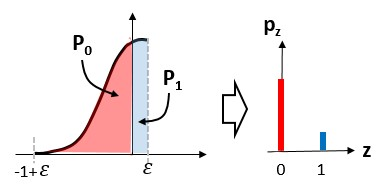
\includegraphics[width=0.7\columnwidth]{pdf.JPG}}
    \caption{Distribution of random variable ($\epsilon- |x_{[i]}-x_{[i+r]}|$) when $x_{[i]}$ is the normalized FFT of Gaussian noise. Half Normal distribution mirrored and shifted by $\epsilon$. The $ceil$ effect, random variable $Z$ is binary with probability of occurrence of one is the red area and the blue area is the probability of occurrence of zero. }
    \label{fig:HND}
\end{figure}
Now, we call $Z$ to the random variable generated by g of Ec. \ref{expresion_g}, $Z=\lceil \epsilon- | X_{i}-X_{i+r}| \rceil$. 
%At this point the random variable $X$ has Raileigth distribution with B according to Eq. \ref{B}.
$Z$ is a random binary variable, the probability of occurrence of 1 is defined as the blue area of Fig. \ref{HND}, and the probability of 0 is the red area in the same figure. We can see that for higher $\epsilon$, greater tolerance to determine the samples similarity, the blue area increases and the red area decreases. This means the probability of $Z$ being one increases and decreases the zero. In Eq. \ref{expresion_g} is $g(i,r)=1$ or $g(i,r)=0$.

%$\lceil \epsilon- | X_{[i]}-X_{[i+r]}| \rceil$ es delta en cero del area que esta desde  $-1+\epsilon$ hasta 0 y deslta en 1 del area de 0 a $\epsilon$.


Then, $L$ is composed of the ratio between two random variables ($L_N$ and $L_D$), each one can be modelled by asymmetric random walks. The steps are formed by $Z1$, $Z2$ and $Z3$ discrete random variables that can be assumed to be independent and identically distributed (iid), all three with the same discrete distribution shown in Fig. \ref{fig:HND}.
The probability of each step is determined by the probability of occurrence shown in Table \ref{tabla}
\begin{figure*}
\center
\begin{tabular}{ c | c  |l|l } 
 \hline
 & $Z1$  $Z2$  $Z3$ & $L_N=(2.Z1-Z2).Z3.Z1$& $L_D=(Z1-Z2).Z3.Z1$ \\ 
  \hline
$p_{z(0)}^3$ & 0  0  0 & 0 & 0  \\ 
$p_{z(0)}^2p_{z(1)}$  & 0  0  1 & 0 & 0  \\ 
$p_{z(0)}^2p_{z(1)}$  & 0  1  0 & 0 & 0 \\ 
$p_{z(0)}p_{z(1)}^2$   & 0  1  1 & 0 & 0  \\ 
$p_{z(0)}^2p_{z(1)}$  & 1  0  0 & 0 & 0  \\ 
$p_{z(0)}p_{z(1)}^2$  & 1  0  1 & 2 $\rightarrow {P_L}_N(2)$ & 1 $\rightarrow {P_L}_D(1)$ \\
$p_{z(0)}p_{z(1)}^2$  & 1  1  0 & 0 & 0 \\ 
$p_{z(1)}^3$  & 1  1  1 & 1 $\rightarrow {P_L}_N(1)$ & 0 \\ 
 \hline
\end{tabular}\label{tabla}
\end{figure*}


$L_N$ random variable increases with step formed by $(2.Z1-Z2).Z3.Z1$ and $L_D$ random variable increases with step formed by $(Z1-Z2).Z3.Z1$. As it can be seen in Table \ref{tabla} 



\begin{figure}[htbp]
    \centerline{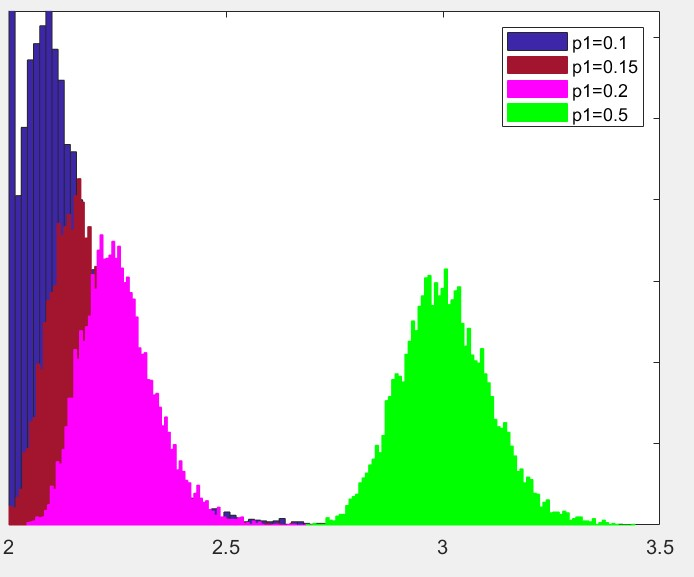
\includegraphics[width=0.7\columnwidth]{pdfL_func_p1.jpg}}
        \centerline{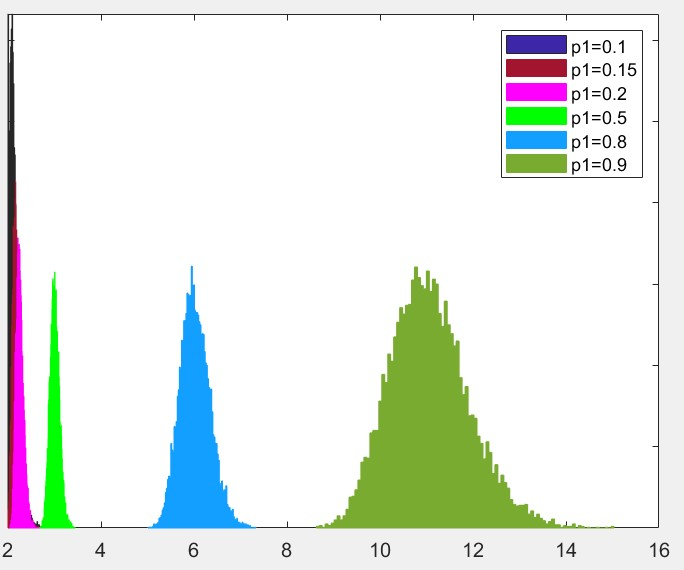
\includegraphics[width=0.7\columnwidth]{pdfL_func_p1_a0p9.jpg}}
    \caption{ }
    \label{pdf_L}
\end{figure}


\begin{figure}[htbp]
    \centerline{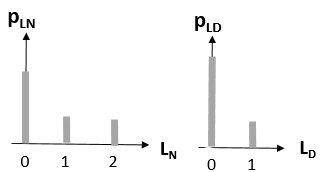
\includegraphics[width=0.7\columnwidth]{PDF_nyd.jpg}}
    \caption{ }
    \label{fig:NyD}
\end{figure}

We can approximate the distribution of $L_N$ and $L_D$ using the Central Limit Theorem. We can say that for a sum large enough: 


$L_N \approx \mathcal{N}({\mu_L}_N,\,{\sigma_L}_N^{2})$ and $L_D \approx \mathcal{N}({\mu_L}_D,\,{\sigma_L}_D^{2})$

The mean value and variance of these random variables can be calculated:

\begin{eqnarray*}
{\mu_L}_N &= &E[\sum_{r=1} ^{N-2} \sum_{i=1} ^{N-r-1} L_N]\\
& =&\sum_{r=1} ^{N-2} \sum_{i=1} ^{N-r-1} E[L_N]\\
&=&\sum_{r=1} ^{N-2} \sum_{i=1} ^{N-r-1} (1.{P_L}_N(1)+2.{P_L}_N(2))\\
&=&\frac{1}{2}(N-2)(N-1)({P_L}_N(1)+2.{P_L}_N(2))\\
&\approx&\frac{1}{2}(N-2)(N-1)(p_1^3+2.p_1^2.p_0)
\end{eqnarray*}

\begin{eqnarray*}
{\sigma_L}_N^2 &= &var[\sum_{r=1} ^{N-2} \sum_{i=1} ^{N-r-1} L_N]\\
& =&\sum_{r=1} ^{N-2} \sum_{i=1} ^{N-r-1} var[L_N]\\
&=&\sum_{r=1} ^{N-2} \sum_{i=1} ^{N-r-1} [(1^2.{P_L}_N(1)+2^2.{P_L}_N(2))\\
& & -({P_L}_N(1)+2.{P_L}_N(2))^2]\\
&=&\frac{1}{2}(N-2)(N-1)[({P_L}_N(1)+4.{P_L}_N(2))\\
& & ({P_L}_N(1)+2.{P_L}_N(2))^2]\\
&\approx&\frac{1}{2}(N-2)(N-1)(p_1^3+4.p_1^2.p_0)
\end{eqnarray*}

E[.] represents the mathematical expectation.

The probability of $L$ is the the joint density of $L_N$ and $L_D$ 
 La variable aleatoria 
 Z es independent and identically distributed (i.i.d.) 
y del denominador que es (Z1-Z2).Z3.Z1 que son dos deltas una en cero y otra en 1.

me da la variable aleatoria L que es la division de la razon entre dos numeros enteros, siempre el numerador es mayor que el denominador.

Eso da gausiano.

Analizo el máximo valor que puede tomar L:
Seria cuando la diagonal mayor esta en 1 y el resto en cero, porque las demas diagonales son menores y ademas se divide por mas.

En este caso solo la diferencia de valores adyacentes esta dentro del  $\epsilon$, el resto son distintos. Entonces con $r<1$ $|x_{[i]}-x_{[i+r]}| >\epsilon$
Para $r=1$ e $i=1$ $g(1,1)=1$ $g(0,1)=0$ y $g(2,1)=1$ =>num=2
Para el resto de $i>1$ y $r=1$ $g(1,1)=1$ $g(0,1)=1$ y $g(2,1)=1$=>el numerador suma 1, entonces:
 
 $num=2+\sum_{i=2} ^{N-2} 1=2+(N-3)=N-1$
 y el denominador:
 
 Para $r=1$ e $i=1$ $g(1,1)=1$ $g(0,1)=0$ y $g(2,1)=1$ =>denom=1
Para el resto de $i>1$ y $r=1$ $g(1,1)=1$ $g(0,1)=1$ y $g(2,1)=1$=>el denominador suma 0, entonces:

 $L_{max}=\frac{2+\sum_{i=2} ^{N-2} 1=2+(N-3)}{1+\sum_{i=2} ^{N-2} 0}=\frac{2+(N-3)}{1}=N-1$

Esto solo se peude dar en el caso que x sea creciente en pasos $\epsilom < \Delta V < 2.\Epsilom$



The folded normal distribution is a probability distribution related to the normal distribution. Given a normally distributed random variable X with mean μ and variance σ2, the random variable Y = |X| has a folded normal distribution.
the half-normal distribution is a fold at the mean of an ordinary normal distribution with mean zero.\cite{Leone1961}




The effect of the quantifier on Gaussian noise was analyzed for the $L_{FFT}$ and $Cov$ sensors. The histograms at the output of the quantifier were qualitatively characterized. It was observed that, for sufficiently high $N$, the random variables at the sensor outputs present distributions that could be approximated to be Gaussian. What is more, the mean value and dispersion of these Gaussian curves remained constant regardless of the noise power at the input. This fact demonstrates the ``blind" behavior of the sensors. This behavior is shown in Fig. \ref{pdf3} where the histogram of sensed noises with two different power are depicted for the three sensors. There, it is emphasized that the variance and the mean value of the Gaussian-like distribution are sensitive to the level of noise power in $DE$ sensor, while $L_{FFT}$ and $Cov$ keep constant both parameters (also shown in Fig. \ref{fig_max}).

%\begin{figure*}
%\center
%\subfloat[$L_{FFT}$]{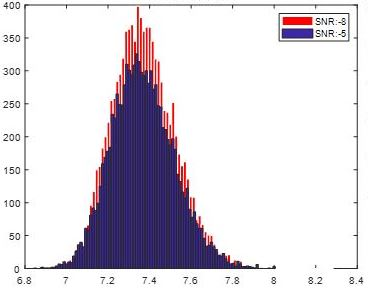
\includegraphics[width =2.3in]{pdf_ruidos_L.JPG}} 
%\subfloat[Cov]{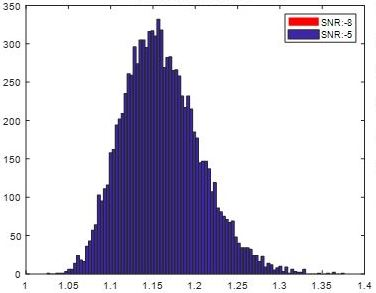
\includegraphics[width = 2.3in]{pdf_ruidos_cov.JPG}}
%\subfloat[DE]{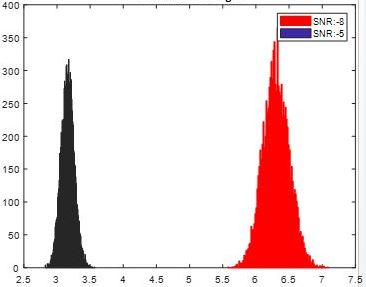
\includegraphics[width = 2.3in]{pdf_ruidos_DE.JPG}}
%\caption{Histogram of the sequence at the detector output $z_k$. Only Gaussian noise is sampled, in blue -8dB and in red -5dB.}
%\label{pdf3}
%\end{figure*}

Therefore, the threshold would be the value of $z_k$ at which the area under the Gaussian-like curve equals the desired $P_{FA}$.
Then, for different values of $N$ the variance and mean values were determined to calculate and tabulate the thresholds.

\section{Results}\label{secResults}

Simulations of the proposed sensor as well as of the energy ($DE$) and covariance ($Cov$) sensors were carried out to compare their performance.
Binary phase modulation (bpsk) was used to emulate the PU signal. Each cycle was sampled $1024$ times at intermediate frequency $1 cycle/symbol$. In all cases, $4096$ samples were taken ($N=4096$).
Figures \ref{fig_max} shows the response of different detectors to SNR. In red a

Figures \ref{pdf1} shows the PDFs obtained at the output of each quantifier when the sensors receive (in blue) only sampled Gaussian noise ($H_0$) and (in red) the PU signal contaminated with Gaussian noise ($H_1$) for SNR of $-13dB$. It can be seen that, in the case of the proposed sensor, the PDFs are the most separated ones, the covariance detector presents the PDFs a little closer and finally, the energy detector is the one with the worst behavior since its PDFs are the closest.
%Fig. \ref{pdf2} shows that a decrease in SNR ($-18dB$) produces the PDFs to get closer to each other, in the three cases.
This information can be seen compacted in Fig. \ref{fig_max}. It is shown the quantifier effect on both Gaussian noise (in blue) and the PU signal contaminated with Gaussian noise (in red) for different SNR values. In this case, $10,000$ runs were calculated for each SNR sensing $N=2,048$ samples. The mean value is shown as a solid line and the colored areas correspond to all the surrogates. In this plot, the PU signal is simulated using 4QAM modulation. Note that for a fixed SNR the graph corresponds to the histograms of Fig. \ref{pdf1}. It is clearly seen how the outputs of $L_{FFT}$ and $Cov$ sensors are independent of the received noise power (blue area). While in the case of the $DE$ sensor the average value of the output varies according to the power of the noise. This fact is crucial for the threshold calculation as we will see in the next subsection.

%\begin{figure*}[h]
%\center
%\subfloat[$L_{FFT}$]{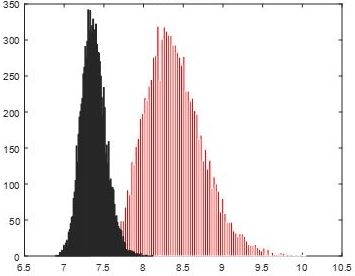
\includegraphics[width = 2.3in]{hist_13dB_L.JPG}} 
%\subfloat[Cov]{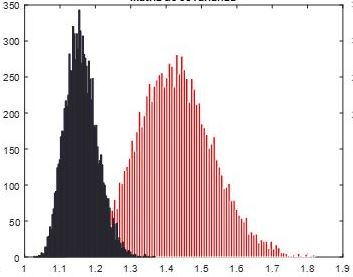
\includegraphics[width = 2.3in]{hist_13dB_cov.JPG}}
%\subfloat[DE]{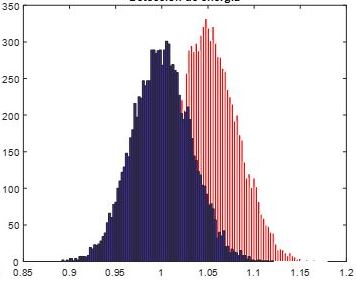
\includegraphics[width = 2.3in]{hist_13dB_DE.JPG}}
%\caption{Histogram of the sequence at the detector output $z_k$. Only Gaussian noise is sampled in blue, primary user signal contaminated with Gaussian noise with SNR=-13dB, in red}
%\label{pdf1}
%\end{figure*}

%\begin{figure*}
%\center
%\subfloat[$L_{FFT}$]{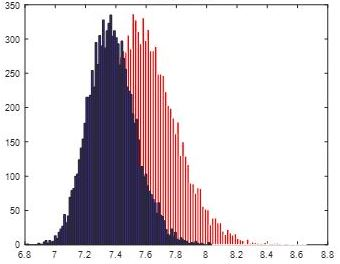
\includegraphics[width = 2in]{hist_18dB_L.JPG}} 
%\subfloat[Cov]{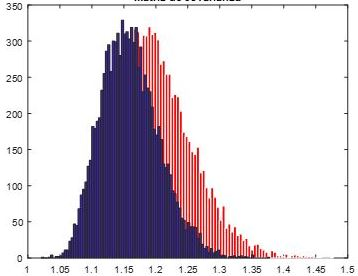
\includegraphics[width = 2in]{hist_18dB_cov.JPG}}
%\subfloat[DE]{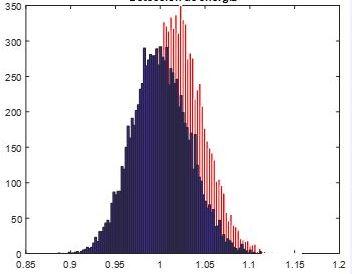
\includegraphics[width = 2in]{hist_18dB_DE.JPG}}
%\caption{Quantifiers vs. SNR Histogram of the sequence at the detector output $z_k$. Only Gaussian noise is sampled in blue, primary user signal contaminated with Gaussian noise with SNR=-18dB, in red.}
%\label{pdf2}
%\end{figure*} 

%\begin{figure*}
%    \center
%    \subfloat[$L_{FFT}$]{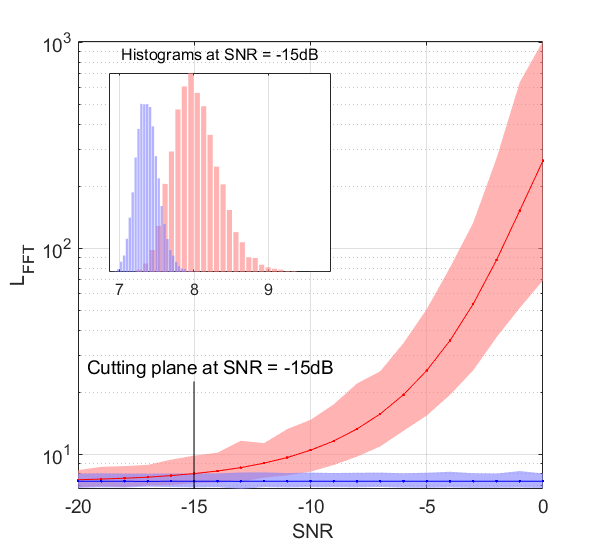
\includegraphics[width = 2.4in]{LvsSNR_1.png}} 
%    \subfloat[Cov]{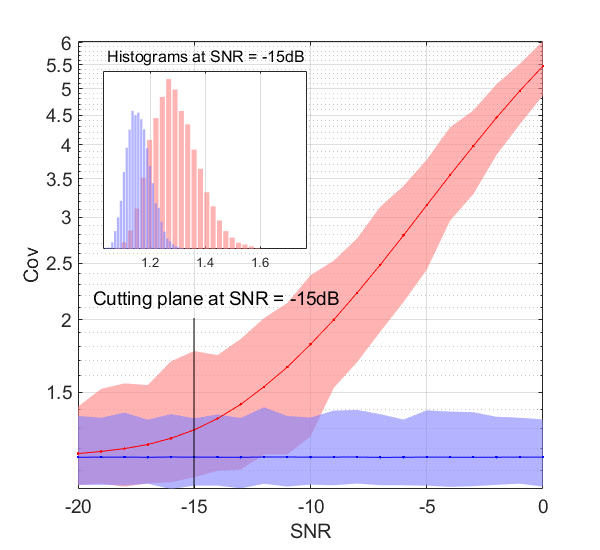
\includegraphics[width = 2.4in]{CovvsSNR_1.png}}
%    \subfloat[DE]{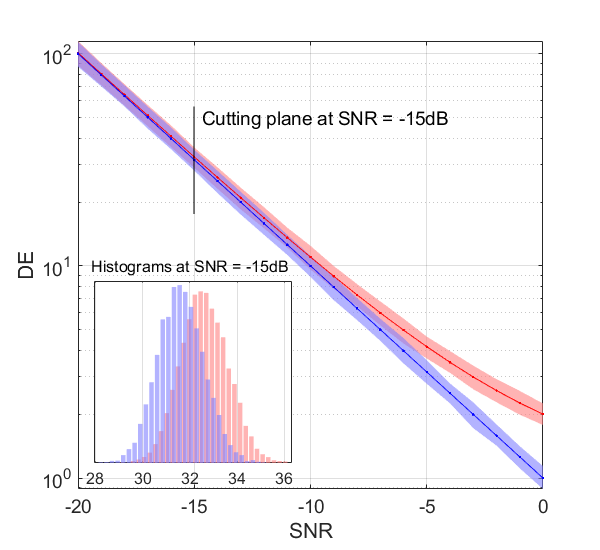
\includegraphics[width = 2.4in]{PotvsSNR_1.png}}
%    \caption{$z_k$ for different SNR. Only Gaussian noise is sampled in blue, primary user signal contaminated with Gaussian noise, in red.}
%    \label{fig_max}
%\end{figure*} 

\begin{figure*}
    \center
    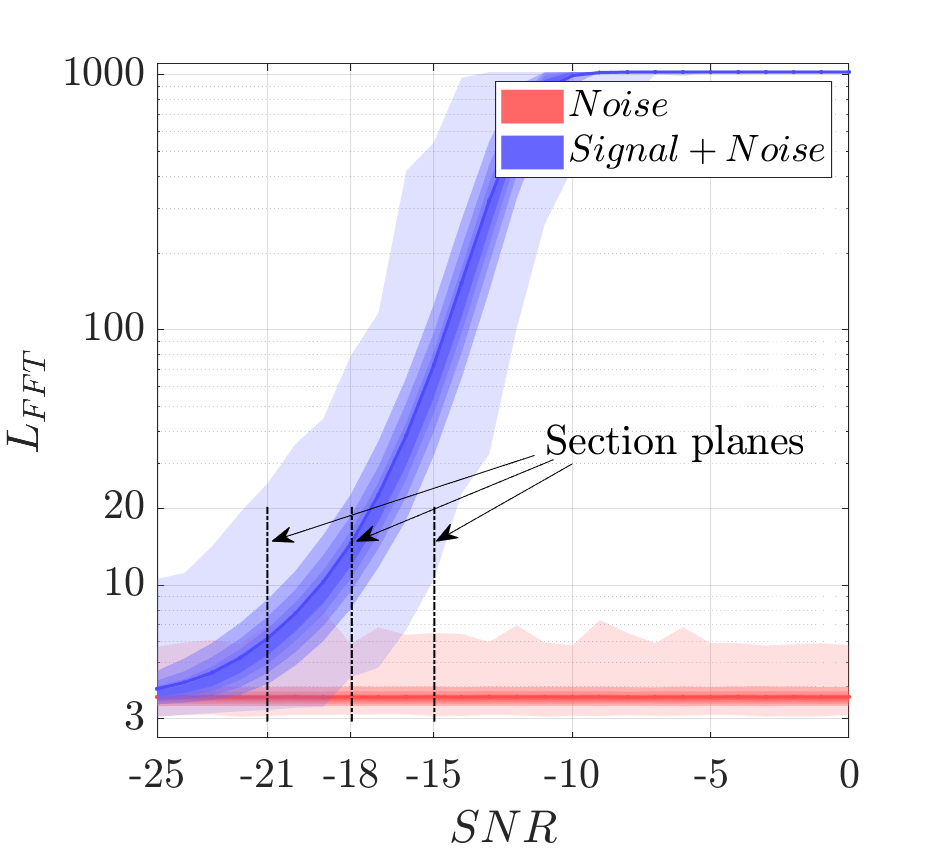
\includegraphics[width = 2.3in]{LvsSNR.png}
    \includegraphics[width = 2.3in]{CovvsSNR.png}
    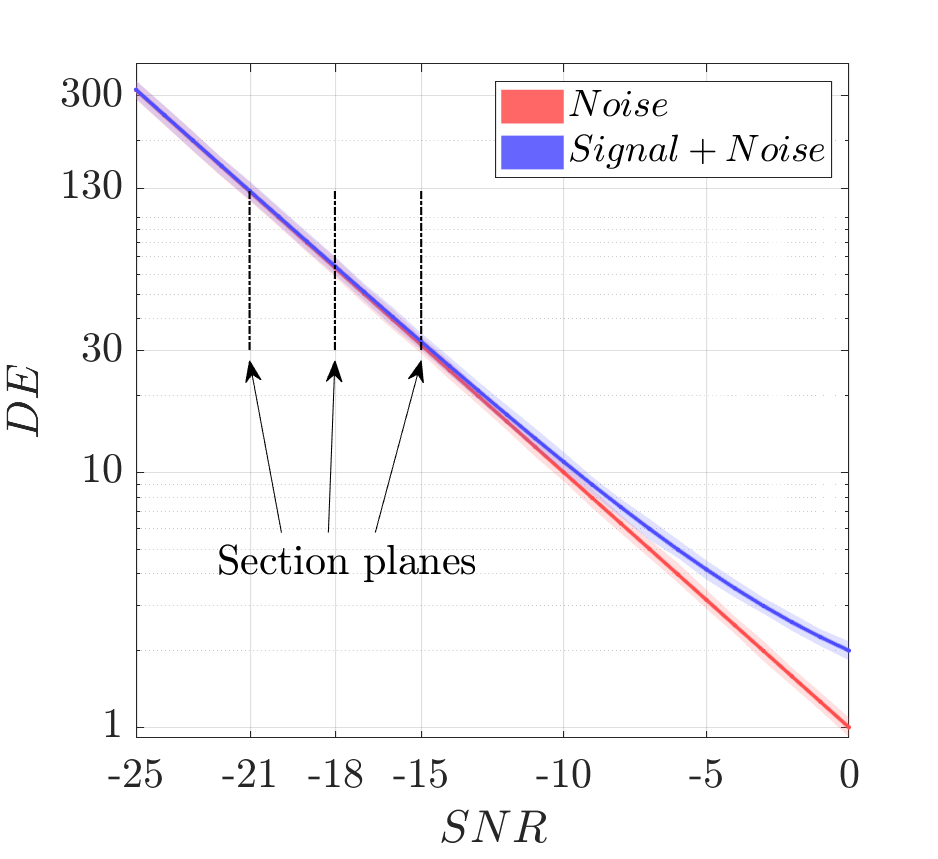
\includegraphics[width = 2.3in]{EvsSNR.png}\\
    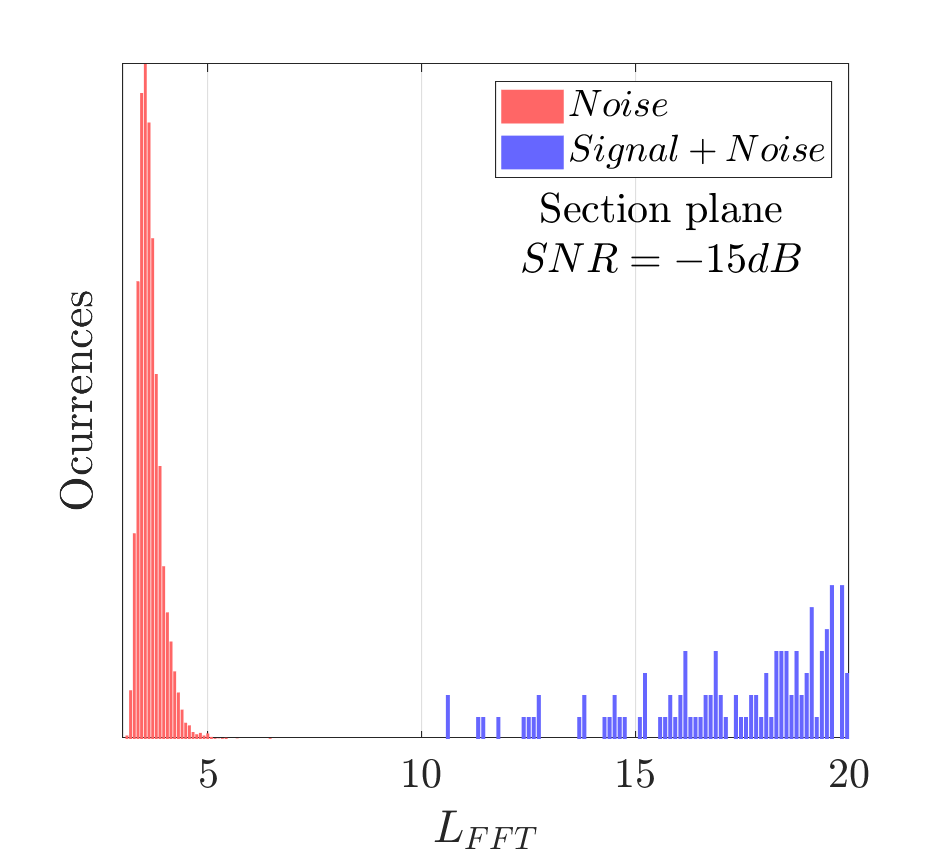
\includegraphics[width = 2.3in]{histL-15db.png}
    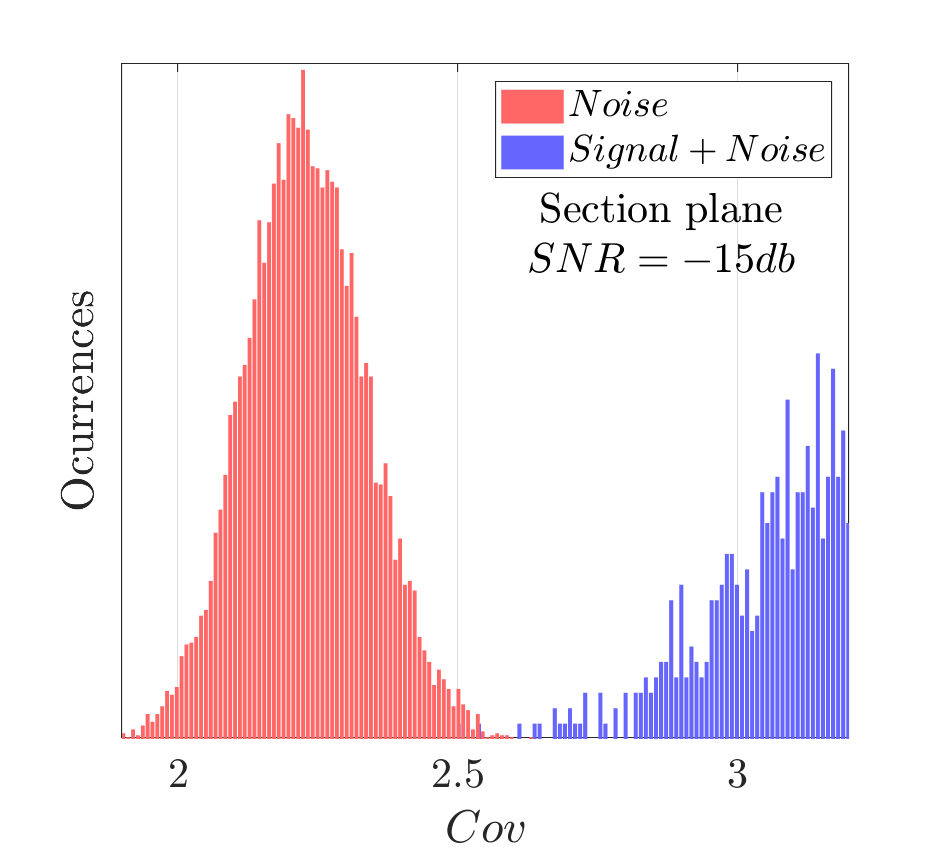
\includegraphics[width = 2.3in]{histCov-15db.png}
    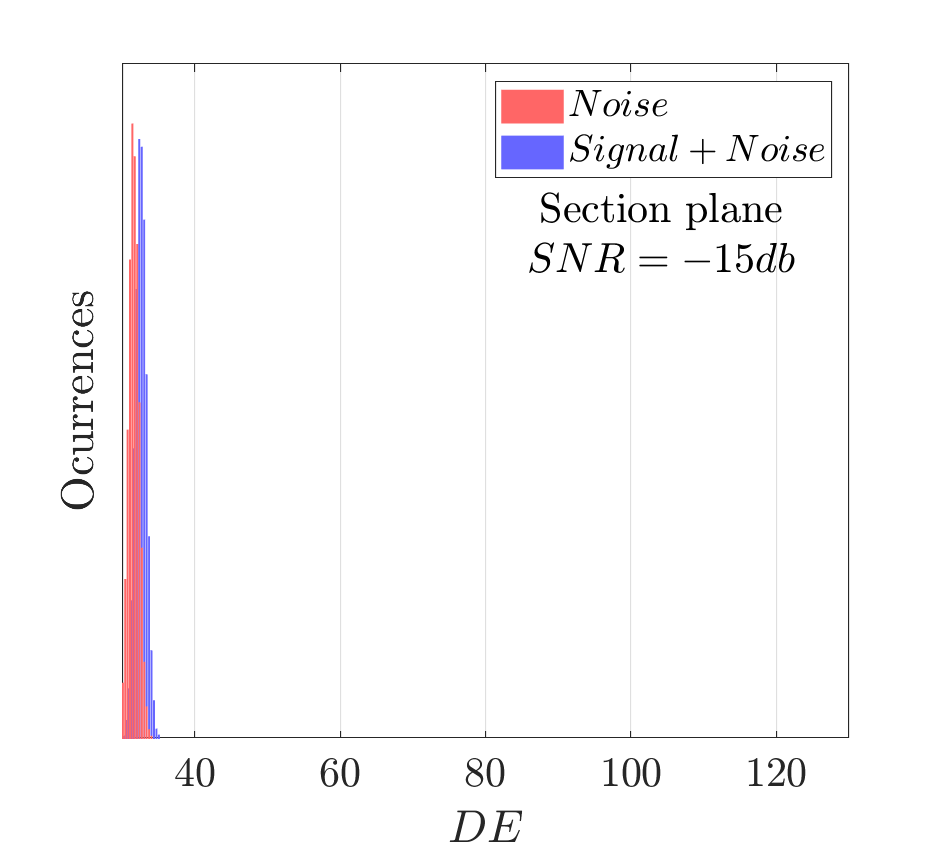
\includegraphics[width = 2.3in]{histE-15db.png}\\
    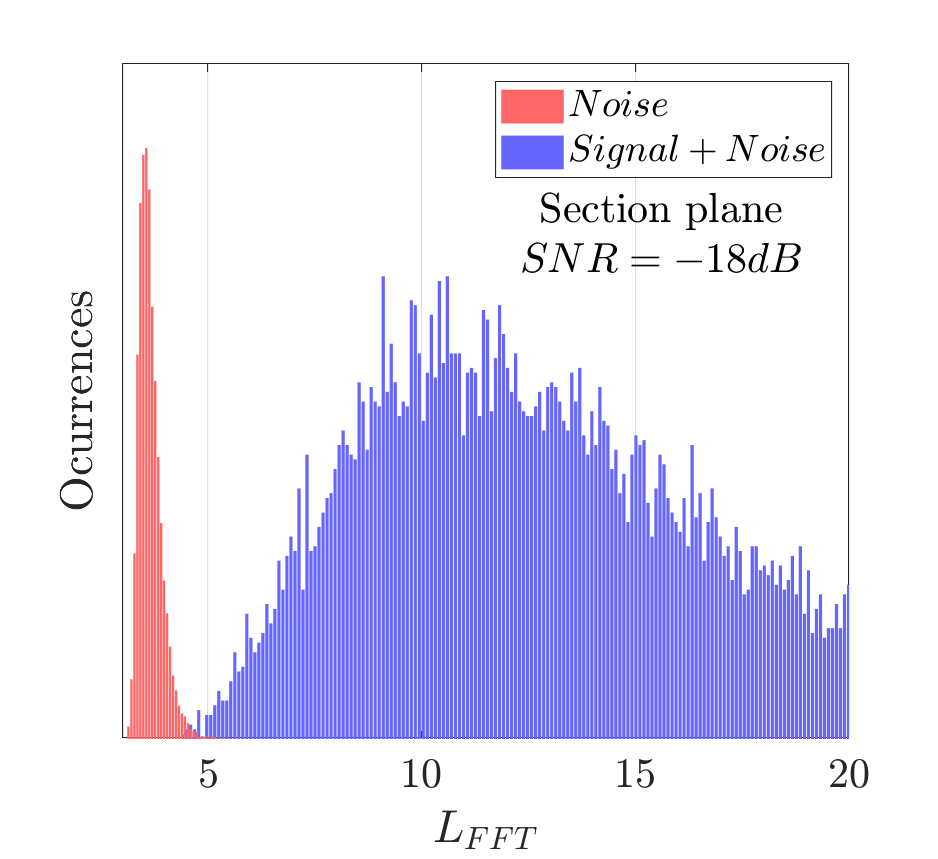
\includegraphics[width = 2.3in]{histL-18db.png} 
    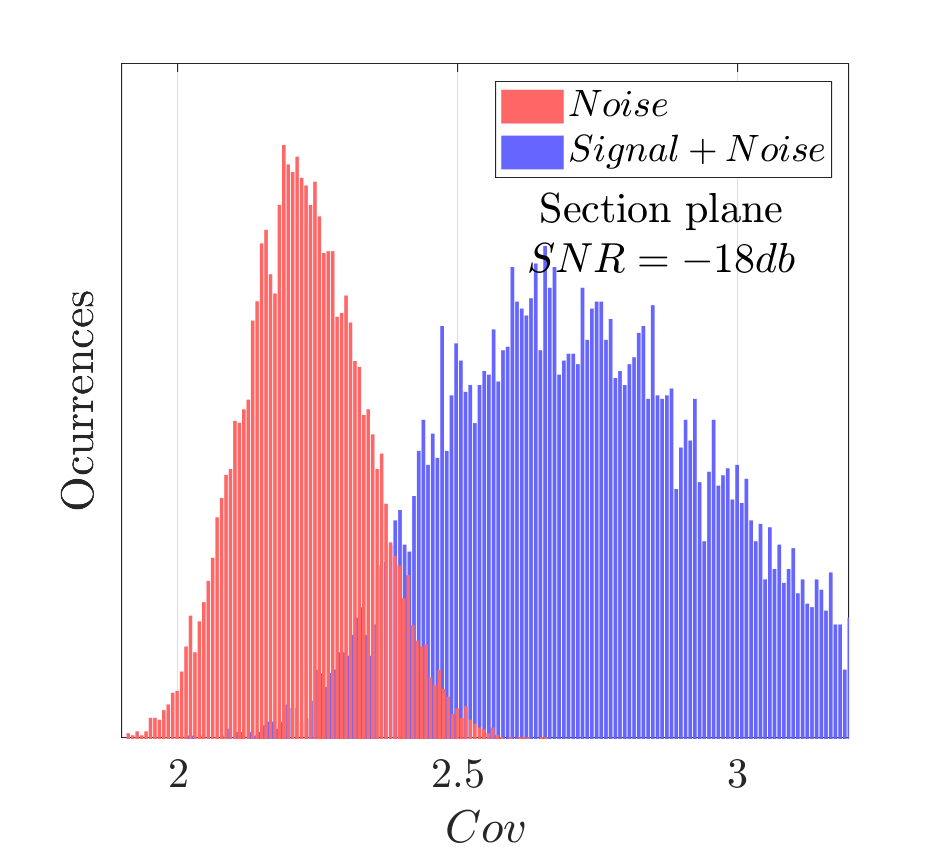
\includegraphics[width = 2.3in]{histCov-18db.png}
    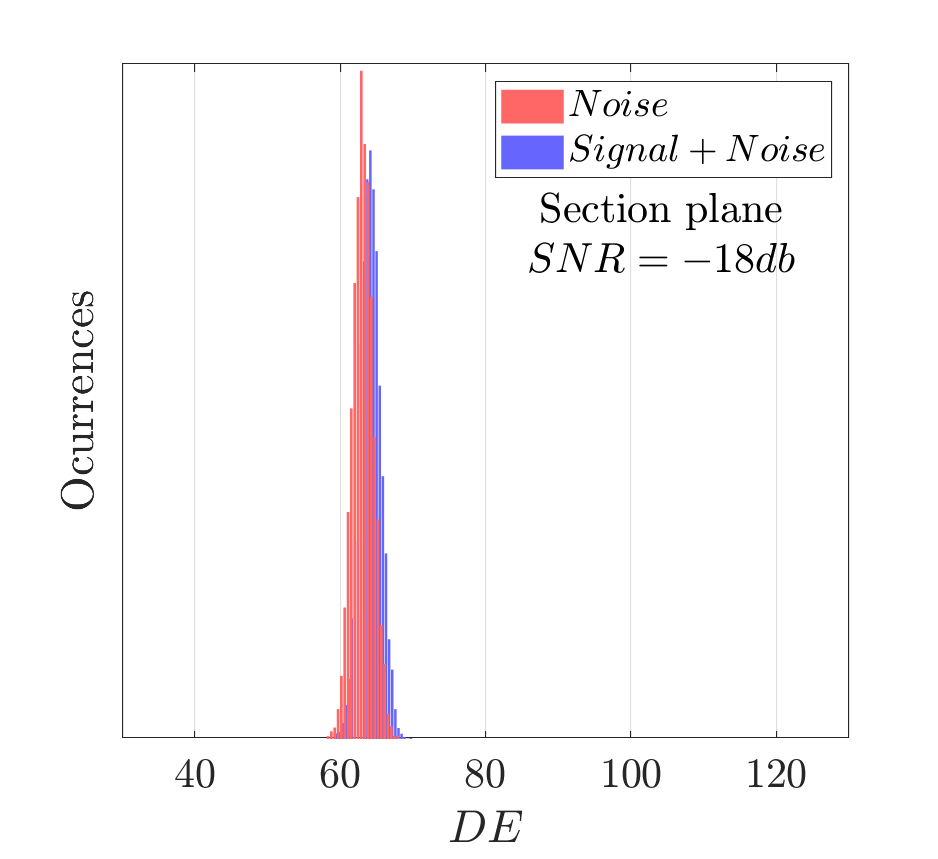
\includegraphics[width = 2.3in]{histE-18db.png}\\
    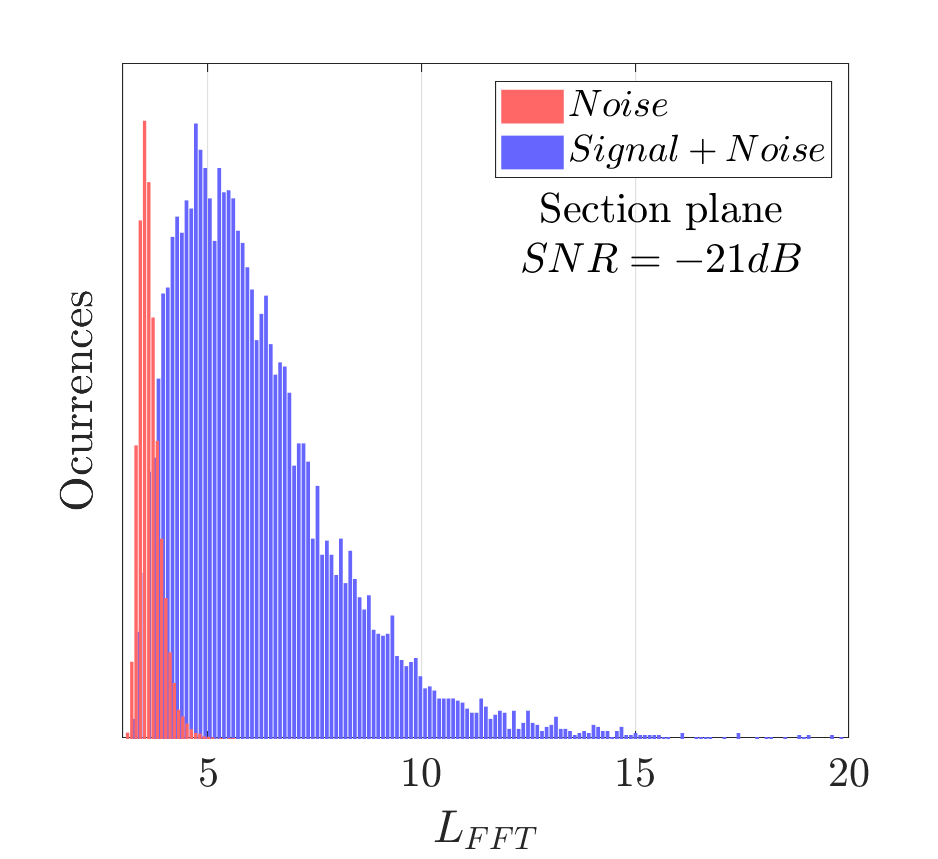
\includegraphics[width = 2.3in]{histL-21db.png} 
    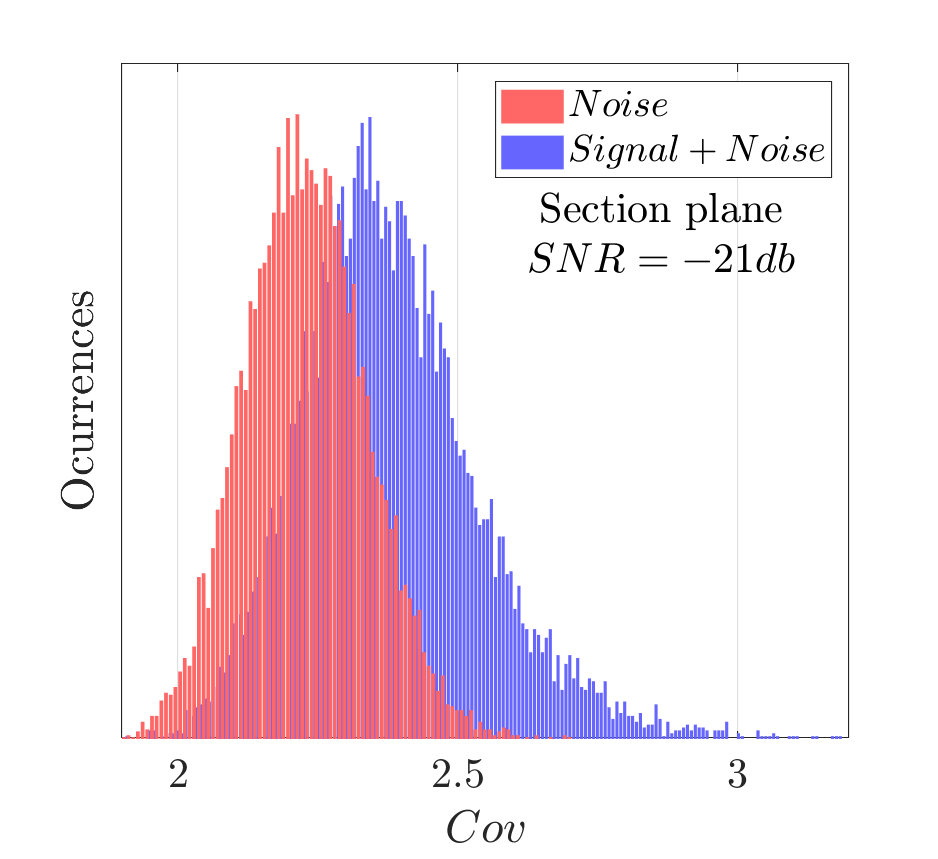
\includegraphics[width = 2.3in]{histCov-21db.png}
    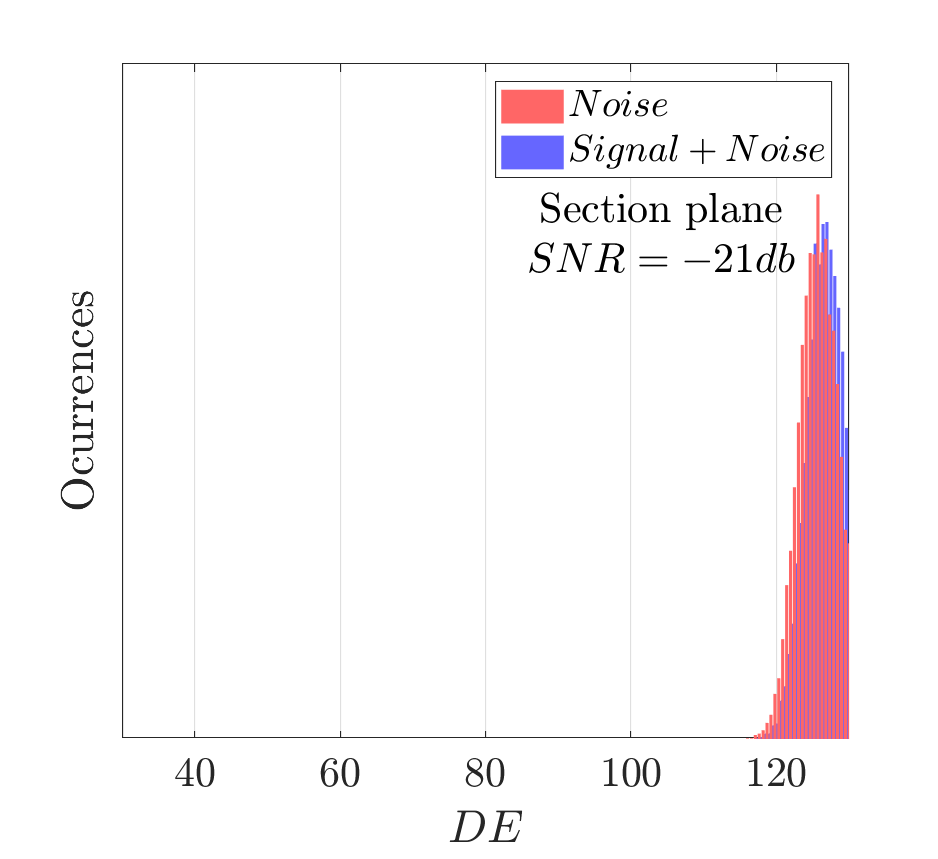
\includegraphics[width = 2.3in]{histE-21db.png}
    \caption{Response of different detectors to SNR. Density plots as function of $SNR$ and histograms for three section planes.}
    \label{fig_max}
\end{figure*} 
%\begin{figure}[htbp]
 %   \centerline{\includegraphics[width=0.9\columnwidth]{ROC_%N2000_SNR-13dB.png}}
 %   \caption{Performance comparison for SNR=-13dB using the %calculated threshold.}
 %   \label{fig:ROC13}
%\end{figure}

%\begin{figure}[htbp]
 %   \centerline{\includegraphics[width=0.9\columnwidth]{ROC_%N2000_SNR-18dB.png}}
 %   \caption{Performance comparison for SNR=-18dB using the %calculated threshold.}
 %   \label{fig:ROC18}
%\end{figure}

\begin{figure}[htbp]
    \centerline{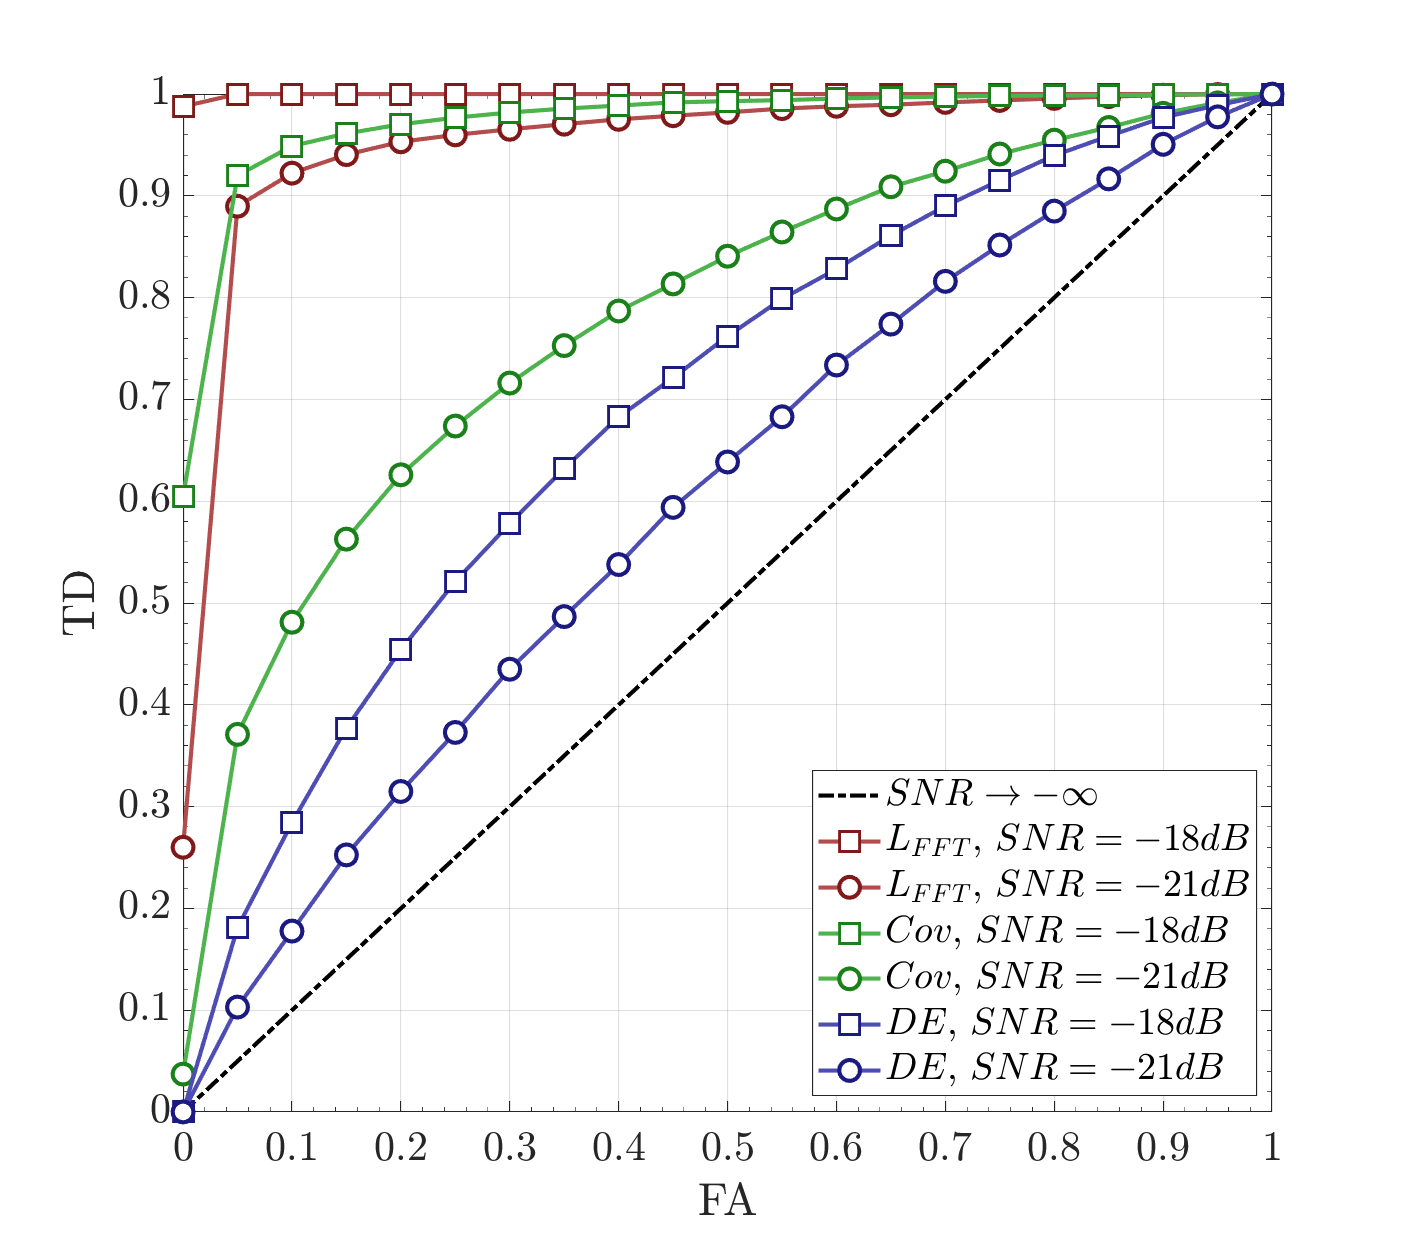
\includegraphics[width=1\columnwidth]{ROC.png}}
    \caption{.}
    \label{fig:ROC_max}
\end{figure}

\subsection{ROC curves}\label{ROC}

From the determined thresholds, the ROC curves were generated to evaluate the performance of the sensors.
% The behavior seen in Figures \ref{pdf1} and \ref{pdf2} is also reflected in the ROC curves of Figures \ref{fig:ROC13} and \ref{fig:ROC18}. On both figures, 
 The curve corresponding to the proposed quantifier is the closest to the ideal curve ($P_{d}=1$ for all $P_{FA}$). When the SNR decreases the three sensors approach the diagonal. There it is also observed that the proposed sensor continues to maintain the best performance.

\section{Conclusions}\label{secConclu}

A blind spectral sensing method for RC based on RP was presented. The proposed detector is based on the measurement of the diagonal lines of the recurrence plots, applied to the FFT of the sampled received signal. The simulations carried out showed that the proposed method outperforms both, the covariance method (also blind) and the energy detection method (the most widely used today).
The next step would be to develop an analytical expression for the calculation of the threshold

\section*{Acknowledgments}

This research was funded by the National Scientific and Technical Research Council (PIP11220170100553CO), Agencia Nacional de Promoción Científica y Tecnológica (PICT2019-3024), Faculty of Engineering of the National University of Mar del Plata (FI-UNMDP).


\bibliographystyle{IEEEtran}
\balance
\bibliography{xbibWEB}

\end{document}
